\documentclass[]{article}
\usepackage[T1]{fontenc}
\usepackage[utf8]{inputenc}
\usepackage[swedish]{babel}
\usepackage[margin=1.7in]{geometry}
\usepackage{mathtools}
\usepackage{graphicx}
\usepackage{listings}



%opening
\title{DD1350 Logik för dataloger \\ Laboration 2}
\author{Erik Ringdahl, erikrin@kth.se \\ Joel Tjärnstig, joelt@kth.se}

\begin{document}

\setlength\parindent{0pt}
\maketitle

\section{Verktygsutveckling}
Programmet börjar med att läsa in modellen, sanningstilldelningslistan, starttillståndet samt formeln. Dessa värden skickas sedan in i ett predikat \texttt{check} tillsammans med en tom lista som håller reda på vilka tillstånd vi har besökt. check verifierar varje delformel rekursivt och börjar innerst. För att göra detta använder check sig av två hjälppredikat, \texttt{check\_all} som rekursivt kollar A-formler, samt \texttt{check\_exist} som rekursivt kollar E-formler.

\clearpage
\section{Modellering}
Vi valde att modellera en förenklad uttagsautomat. En användare möts först av en välkomstskärm. Användaren verifieras genom att ange sin pinkod. Om pinkoden är fel, bes användaren ange den igen. Om användaren anger rätt pinkod får ett belopp anges. Om beloppet inte kan tas ut får användaren skriva ett nytt belopp. Om beloppet finns tillgängligt tas pengarna ut och uttagsautomaten återgår till välkomstskärmen. Användaren kan även närsomhelst avbryta uttaget och återgå till välkomstskärmen.

\subsection{Tillståndsgraf}
Vi har 5 olika tillstånd (\textbf{Welcome Screen, Verify, Retry, Select Amount, Withdraw Money}) och 4 atomer (\texttt{Pin Entered, Failed, Verified, Valid Amount}).

\begin{figure}[h]
\centering
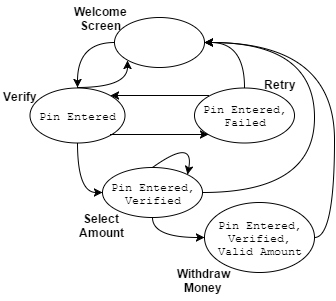
\includegraphics[width=0.75\linewidth]{modell}
\caption{Tillståndsgraf för uttagsautomat}
\label{fig:modell}
\end{figure}

\clearpage
\subsection{Prolog-kompatibel representation}
\begin{verbatim}
% States are ws(welcome screen), ve(verify), re(retry), 
% sa(select amount) and wm(withdraw money).
[
 [ws, [ve]],
 [ve, [ws, ve, re, sa]],
 [re, [ws, ve]],
 [sa, [ws, sa, wm]],
 [wm, [ws]]
].

% Labeling
[
 [ws, []],
 [ve, [pe]],
 [re, [pe, f]],
 [sa, [pe, v]],
 [wm, [pe, v, va]]
].
\end{verbatim}

\clearpage
\section{Specifiering}

\subsection{Hållbar systemegenskap}
Det finns en stig där så småningom det går att ta ut pengar.\\
\texttt{ef(and(and(pe,v),va))}

\subsection{Ohållbar systemegenskap}
Det finns en stig där något av nästa steg inte är välkomstskärmen.\\
\texttt{ef(not(ex(not(pe))))}

\section{Predikat}
\begin{description}
	\item[\texttt{verify -}] sant när bevisfilen kan läsas på ett korrekt sätt samt när formeln är sann.
	
	\item[\texttt{check -}] sant när formeln samt alla underliggande rekursiva anrop är sanna.
	
	\item[\texttt{check\_all -}] sant då basfallet gäller, dvs när grannlistan är tom. Eller när formeln gäller för alla grannar i listan.
	
	\item[\texttt{check\_exist -}] sant då basfallet inte gäller, dvs när grannlistan inte är tom. Eller när formeln gäller för någon granne i listan.
	
	\end{description}

\section{Verifiering}
\subsection{Systemegenskaper}
\begin{description}
	\item[Hållbar] Eftersom det finns en stig där \texttt{pe,v,a} kommer att vara sanna, nämligen i \texttt{ws} ska egenskapen returnera sant, vilket den gjorde.
	
	\item[Ohållbar] Eftersom alla tillstånd kan gå över till \texttt{ws} alltså då \texttt{pe} inte är sann ska egenskapen returnerna falskt, vilket den gjorde.
\end{description}

\subsection{Givna Testfall}
Modellproveraren klarade samtliga 732 givna testfall.

\clearpage
\section*{Appendix}
\appendix

\section{Källkod}

\begin{verbatim}
	% For SICStus, uncomment line below: (needed for member/2)
	%:- use_module(library(lists)).
	
	verify(Input) :-
	see(Input), read(T), read(L), read(S), read(F), seen,
	check(T, L, S, [], F).
	
	% check(T, L, S, U, F)
	% T - The transitions in form of adjacency lists
	% L - The labeling
	% S - Current state
	% U - Currently recorded states
	% F - CTL Formula to check.
	%
	% Should evaluate to true iff the sequent below is valid.
	%
	% (T,L), S |- F
	% U
	% To execute: consult(’your_file.pl’). verify(’input.txt’).
	
	% Literals - check for the state S and its axiom list that is does contain X
	check(_, L, S, [], X) :-
	member([S,Z],L), 
	member(X, Z).
	
	%neg(X) - check for the state S and its axiom list that is does NOT contain X
	check(_, L, S, [], neg(X)) :-
	member([S,Z],L), 
	\+ member(X, Z).
	
	% And - check for the state S and its axiom list if F AND G is valid
	check(T, L, S, [], and(F,G)) :-
	check(T, L, S, [], F),
	check(T, L, S, [], G).
	
	% Or - check for the state S and its axiom list if F OR G is valid
	check(T, L, S, [], or(F,G)) :- 
	check(T, L, S, [], F);
	check(T, L, S, [], G).
	
	% AX F - all next states satisfies F
	check(T, L, S, [], ax(F)) :-
	member([S, Z], T), % Fetch list Z of neighbors to S from tranistions T
	check_all(T, L, Z, [], F, F). % Check for all neighbours Z
	
	% AG F - F is satisfied in every future state
	% Success if loop is found
	check(T, L, S, U, ag(F)):-
	member(S, U).
	check(T, L, S, U, ag(F)) :-
	\+ member(S, U),
	check(T, L, S, [], F), % check if true in current state S
	member([S, Z], T), % Fetch list Z of neighbors to S from tranistions T
	check_all(T, L, Z, [S|U], F, ag(F)). % Check for all neighbours Z, Add S to recorded states U
	
	% AF F - all paths will satisfy F eventually
	% Fail if loop found
	check(T, L, S, U, af(F)):-
	\+ member(S, U),
	check(T, L, S, [], F).
	
	check(T, L, S, U, af(F)) :- % check if true in current state S
	\+ member(S, U),
	member([S, Z], T), % Fetch list Z of neighbors to S from tranistions T
	check_all(T, L, Z, [S|U], F, af(F)). % Check for all neighbours Z, Add S to recorded states U
	
	% EG - check if some path will always satisfy F
	check(T, L, S, U, eg(F)):-
	member(S, U).
	check(T, L, S, U, eg(F)) :-
	\+ member(S, U),
	check(T, L, S, [], F), % check if true in current state S
	member([S, Z], T), % Fetch list Z of neighbors to S from tranistions T
	check_exist(T, L, Z, [S|U], F, eg(F)). % Check for all neighbours Z, Add S to recorded states U
	
	
	% EF F - some path will satisfy F eventually
	check(T, L, S, U, ef(F)):-
	\+ member(S, U),
	check(T, L, S, [], F). % check if true in current state S
	check(T, L, S, U, ef(F)) :-
	\+ member(S, U),
	member([S, Z], T), % Fetch list Z of neighbors to S from tranistions T
	check_exist(T, L, Z, [S|U], F, ef(F)). % Check for all neighbours Z, Add S to recorded states U
	
	% EX F - some next state will satify F
	check(T, L, S, [], ex(F)) :-
	member([S, Z], T), % Fetch list Z of neighbors to S from tranistions T
	check_exist(T, L, Z, [], F, F). % Check for all neighbours Z
	
	% Help predicate for A-formulas
	check_all(_,_,[],_,_,_). % All neighbours check
	check_all(T, L, [H|TAIL], U, X, A) :-
	check(T, L, H, U, A), % True in the head H of the neighbour list
	check_all(T, L, TAIL, U, X, A). %True in the TAIL of the neighbour list
	
	% Help predicate for E-formulas
	check_exist(_,_,[],_,_,_):- fail. %Fails if list is empty
	check_exist(T, L, [H|TAIL], U, X, A) :-
	check(T, L, H, U, A); %True and the head H of the neighbour list
	check_exist(T, L, TAIL, U, X, A). % or true in the TAIL of the neighbour list
	
\end{verbatim}



\end{document}